%%%%%%%%%%%%%%%%%%%%%%%%%%%%%%%%%%%%%%%%%%%%%%%%%%%%%%%%%%%%%%%%%%%%%%
\begin{frame}[fragile]\frametitle{}
\begin{center}
{\Large Queue}
\end{center}

\end{frame}

\begin{frame}
	\frametitle{The Queue ADT}
	\begin{overlayarea}{\textwidth}{\textheight}
		\begin{block}{The Queue}
			\begin{itemize}
				\item \texttt{size()} (or \texttt{len(s)}) to get the number of items in the queue.
				\item \texttt{enqueue(item)} to add something to the queue.
					\pause
				\item \texttt{dequeue()} to remove the first element from the queue.
				\item \texttt{peek()} to view the first element of the queue.
			\end{itemize}
		\end{block}	
		\pause
		\begin{block}{Data structure?}
			What kind of data structure should we use to implement a Queue?
				\only<3>{
				\begin{enumerate}[A.]
					\item An array
					\item A python list
					\item A linked list
					\item A dict
				\end{enumerate}
			}
		\end{block}
		\pause
		\begin{block}{One end only}
			Only removing on one end and adding on the other? Seems like a DLL will do.
		\end{block}
	\end{overlayarea}
\end{frame}

\begin{frame}
	\frametitle{Implementing a Linked-List based Queue}
	\begin{overlayarea}{\textwidth}{\textheight}
			\begin{tabular}{r | c c}
				Queue operation & DLL operation & Time Complexity \\
				\midrule
				\texttt{size} & \only<2->{\texttt{size} & $O(1)$} \\
				\texttt{enqueue} & \only<2->{\texttt{add\_last} & $O(1)$} \\
				\texttt{dequeue}  & \only<2->{\texttt{remove\_first} & $O(1)$} \\
				\texttt{peek}  & \only<2->{\texttt{head} & $O(1)$} \\
			\end{tabular}
		
			\begin{columns}[t]
				\column{0.455\textwidth}
			\only<3->{
			\begin{block}{Arrays}
				Could we also do this using an array-based list?	
			\end{block}
		}
			\only<5->{
			\begin{block}{SLL}
				What about an SLL?
			\end{block}
		}
				\column{0.455\textwidth}
				\only<4->{
				\begin{block}{No more growing}
					Sure, but only for fixed capacity queues.
				\end{block}
				}
				\only<6->{
				\begin{block}{Eeyore}
					Only if we have the tail pointer.
				\end{block}
				}
		
			\end{columns}
	\end{overlayarea}
\end{frame}

\begin{frame}
	\frametitle{Snake games}
	\framesubtitle{Nostalgia overload}
	\begin{center}
		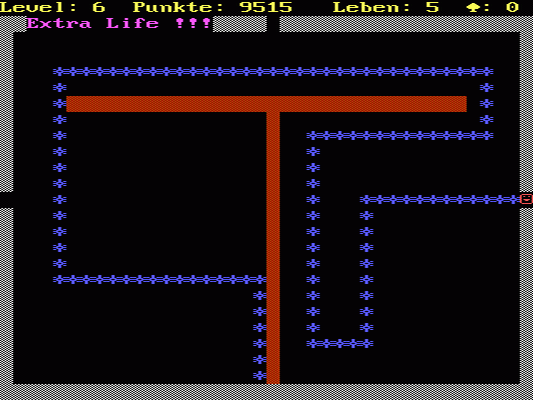
\includegraphics[width=0.6\textwidth]{images/snake.png}\\
		\hspace*{15pt}\hbox{\scriptsize Image By:\thinspace{\itshape Thomas Jensen}}
	\end{center}
	% https://commons.wikimedia.org/wiki/File:Cgasnake.png 
\end{frame}

\begin{frame}
	\frametitle{Why a queue}
		\begin{block}{In snake...}
			\begin{itemize}
				\item In snake, the body of the snake follows the head.
					\pause
				\item If we first go left, then right, then every part of the body also needs to go first left then right.
					\pause
				\item This is like a queue!
			\end{itemize}
		\end{block}	
		\pause
			\begin{block}{Many others?}
				But of course there are many other real-world examples.
				\begin{itemize}
					\item Ticket counters,
					\item Traffic jams,
					\item Coffee machines and printers,
					\item Take-out restaurants,
					\item etc.
				\end{itemize}
			\end{block}	
\end{frame}

\begin{frame}
	\frametitle{Double-Ended Queues}

	\begin{center}
		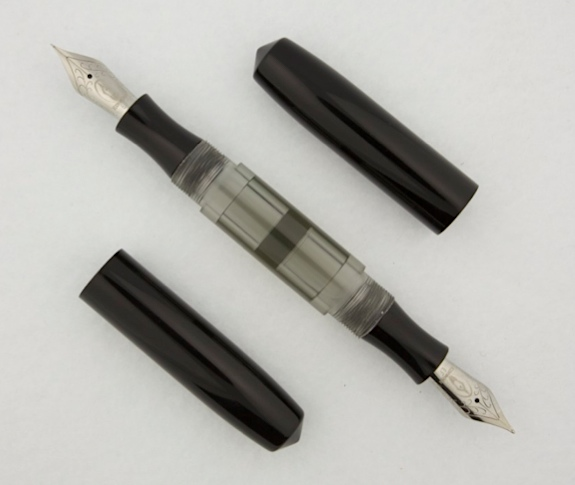
\includegraphics[width=0.5\textwidth]{images/de.jpg}\\
		\hspace*{15pt}\hbox{\scriptsize Image By:\thinspace{\itshape Chris Lott}}
		% https://www.flickr.com/photos/fncll/9824392125
	\end{center}
\end{frame}

\begin{frame}
	\frametitle{Deques}
		\begin{block}{Deques}
			Deques, or Double-Ended Queues, allow both FIFO and LIFO operations in $O(1)$ time.
		\end{block}		
		\pause
		\begin{block}{Hang on...}
			Doesn't that sound familiar?	
		\end{block}
		\pause
		\begin{block}{Back to DLL}
			This is exactly what a DLL offers!
		\end{block}
\end{frame}

\begin{frame}
	\frametitle{\texttt{deque}}
	
	In python we can use a \texttt{deque} called \texttt{d} on which:
	\begin{itemize}
		\item We can \textit{push} with \texttt{d.append}.
		\item We can \textit{pop} with \texttt{d.pop}.
		\item We can \textit{top} with \texttt{d[-1]}
			\pause
		\item We can \textit{enqueue} with \texttt{d.append}.
		\item We can \textit{dequeue} with \texttt{d.popleft}.
		\item We can \textit{peek} with \texttt{d[0]}
			\pause
		\item Oh yeah and if you want, you can also add to the left with \texttt{appendleft}
	\end{itemize}
\end{frame}


%%%%%%%%%%%%%%%%%%%%%%%%%%%%%%%%%%%%%%%%%%%%%%%%%%%%%%%%%%%%%%%%%%%%%%
\begin{frame}[fragile]\frametitle{}
\begin{center}
{\Large Stack}
\end{center}

\end{frame}


\begin{frame}
	\frametitle{Stacks}
	\begin{center}
		
\includegraphics[width=0.4\textwidth]{images/stack_of_books.png}\\
		\hspace*{15pt}\hbox{\scriptsize Image from \thinspace{\itshape Pixabay}}
		% https://pixabay.com/en/books-stacked-pile-stacks-25159/
	\end{center}
\end{frame}

\begin{frame}
	\frametitle{Me and my books}
	\framesubtitle{A life-long story}

	\begin{columns}
		\column{0.455\textwidth}
			\begin{center}
				\alt<4->{
					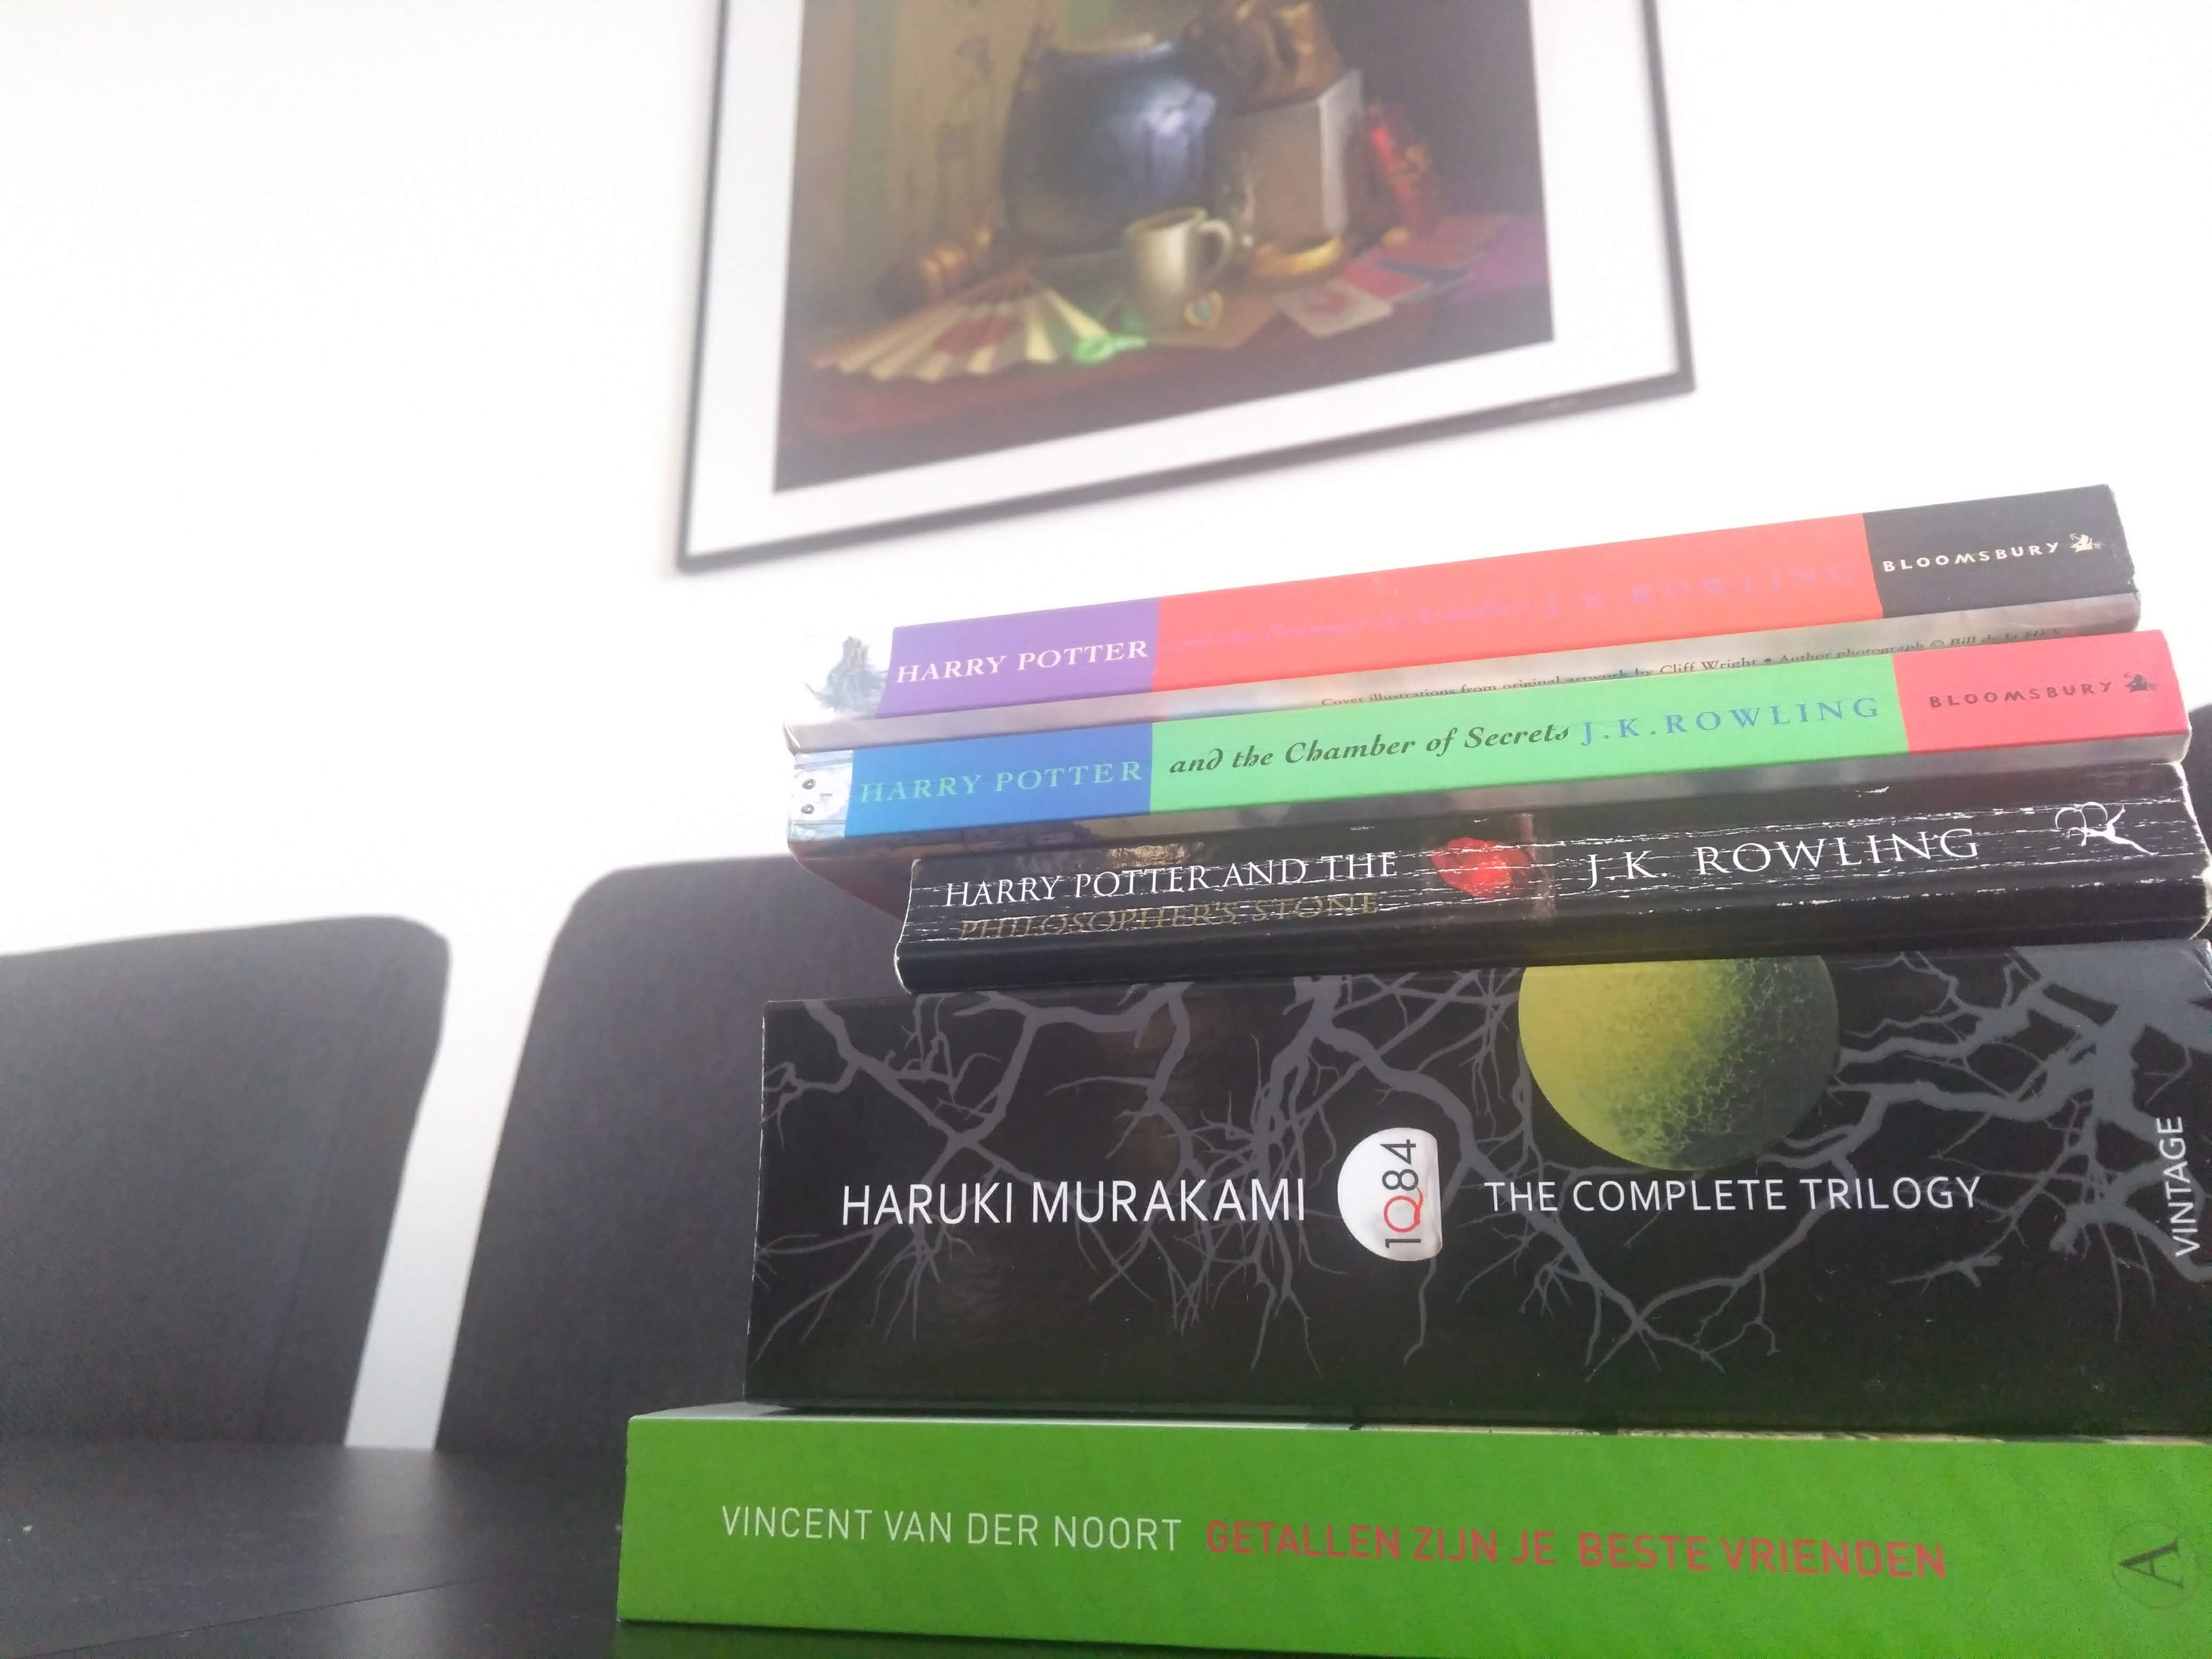
\includegraphics[width=\textwidth]{images/stack_read.jpg}\\
					}{
					
\includegraphics[width=\textwidth]{images/stack_unread.jpg}\\
					}
				\hspace*{15pt}\hbox{\scriptsize Image By:\thinspace{\itshape Stefan Hugtenburg}}
				\hspace*{15pt}\hbox{\scriptsize Bookcovers and picture in the back by others}
			\end{center}
		\column{0.455\textwidth}
		\begin{itemize}
			\item This is how I used to store books I still wanted to read.
				\pause
			\item A nice \alert{stack} of books, with new ones going on the top.
				\pause
			\item After finishing one, I would take the next one from the top.
				\pause
			\item So after a few weeks\dots
				\pause
			\item This uses the \alert{LIFO}-principle.
		\end{itemize}
	\end{columns}
\end{frame}

\begin{frame}
	\frametitle{The what!?}
	\framesubtitle{LIFO}
	
		\begin{block}{LIFO}
			The \textit{Last-In-First-Out}, or LIFO, principle is the working of a stack.\\
			\pause
			The last thing we've added to the stack is the first thing we take out.\\
			\pause
			Similarly the first we have added to the stack, is the last to be taken out.
		\end{block}	
\end{frame}

\begin{frame}
	\frametitle{The Stack ADT}
	\begin{overlayarea}{\textwidth}{\textheight}
		\only<1>{
			\begin{block}{ADT}
				An ADT, or Abstract Data Type, is a description of the behaviour of a data structure.
			\end{block}	
		}
		\pause
			\begin{block}{The Stack}
				\begin{itemize}
					\item \texttt{size()} (or \texttt{len(s)}) to get the number of items in the stack.
					\item \texttt{push(item)} to add something to the stack.
						\pause
					\item \texttt{pop()} to remove the top element from the stack.
					\item \texttt{top()} to view the top element of the stack.
				\end{itemize}
			\end{block}	
			\pause
			\begin{block}{Data structure?}
				What kind of data structure should we use to implement a Stack?
				\only<4>{
				\begin{enumerate}[A.]
					\item An array
					\item A python list
					\item A linked list
					\item A dict
				\end{enumerate}
			}
			\end{block}
			\pause
			\begin{block}{One end only}
				Only removing and adding on one end? Seems like a DLL will do.
			\end{block}
	\end{overlayarea}
\end{frame}

\begin{frame}
	\frametitle{Implementing a Linked-List based Stack}
	\begin{overlayarea}{\textwidth}{\textheight}
			\begin{tabular}{r | c c}
				Stack operation & DLL operation & Time Complexity \\
				\midrule
				\texttt{size} & \only<2->{\texttt{size} & $O(1)$} \\
				\texttt{push} & \only<2->{\texttt{add\_last} & $O(1)$} \\
				\texttt{pop}  & \only<2->{\texttt{remove\_last} & $O(1)$} \\
				\texttt{top}  & \only<2->{\texttt{tail} & $O(1)$} \\
			\end{tabular}
		
			\begin{columns}[t]
				\column{0.455\textwidth}
			\only<3->{
			\begin{block}{Arrays}
				Could we also do this using an array-based list?	
			\end{block}
		}
			\only<5->{
			\begin{block}{SLL}
				What about an SLL?
			\end{block}
		}
				\column{0.455\textwidth}
				\only<4->{
				\begin{block}{Amortised}
					Sure, but it's only amortised $O(1)$. So why would we?
				\end{block}
				}
				\only<6->{
				\begin{block}{Front = Back}
					Sure, but we add and remove from the front!
				\end{block}
				}
		
			\end{columns}
	\end{overlayarea}
\end{frame}

